  \section{Sockets}  
  
     Sockets sind nach \cite{defsockets} folgenderma�en definiert. 
    \begin{quotation}
      Sockets is a method for communication between a client program and a server program in a network. 
      A socket is defined as the endpoint in a connection. Sockets are created and used with a set 
      of programming requests or function calls sometimes called the sockets application 
      programming interface (API). The most common sockets API is the Berkeley UNIX C language 
      interface for sockets. Sockets can also be used for communication between processes 
      within the same computer. 
    \end{quotation}
    
    Ein Socket ist also eine Schnittstelle zwischen einem Prozess 
    und einem Transportprotokoll. Letzteres kann z.B. TCP oder UDP sein. 
    Das Socket-Prinzip entspricht dem von File-Deskriptoren. 
    Dort repr�sentiert nach dem �ffnen einer Datei ein Handle die Verbindung
    zu dieser Datei und unter Angabe des Handles ist der Lese- oder Schreibzugriff m�glich. 
    Bei Sockets geht es jedoch nicht um physikalische Dateien sondern um Kommunikationskan�le, �ber 
    die Daten gesendet und empfangen werden k�nnen.

    Socket-Schnittstellen sind zwar von keiner Institution genormt, 
    stellen aber einen de-facto- bzw. Industriestandard dar, was zum einen daran liegen d�rfte, 
    dass sie leicht verst�ndlich sind, zum anderen f�gen sie sich ausgesprochen 
    harmonisch in die UNIX-Umwelt ein. Eine Variante der Socket-Schnittstelle wurde von 
    Microsoft und verschiedenen anderen Firmen unter der Bezeichnung WinSock in das 
    Schnittstellenangebot der Windows Open Service Architecture (WOSA) aufgenommen und 
    d�rfte damit auch ein etablierter Standard in der PC-Welt sein.
    
    \subsection{Arten von Sockets}
    
      Sockets stellen eine allgemeine Form der Kommunikation zwischen Dateien, Prozessen usw. dar.
      Schon allein die Verwendung unterschiedlicher �bertragungsprotokolle 
      spezifiziert unterschiedliche Anwendungsgebiete. 
      Folgende Arten von Sockets werden darum unterschieden:
      
      \begin{itemize}
        \item Stream Socket \\
              Stream Sockets setzen auf dem verbindungsorientierten TCP auf. Er ist
              langsamer als ein Datagramm Socket, aber daf�r wird die �bertragungskontrolle 
              gew�hrleistet.
        \item Datagram Socket \\
              Datagram Sockets setzen auf dem verbindungslos orientierten User Datagram Protocol (UDP) auf.
              Das gro�e Problem dabei ist, dass die �bertragungskontrolle fehlt. Ansonsten ist die 
              �bertragungsart sehr schnell, falls die Pakete ankommen und erzeugt kaum
              Overhead.
        \item Raw Socket \\
              Ein Raw Socket ist ein spezieller Socket. Er erm�glicht dem Benutzer den 
              direkten Zugang zum Netzwerk, 
              indem man eigene Pakete einspeisen kann. Raw Socket benutzen z.B. das Protokoll ICMP. 
              Sie sind sehr 
              schnell, da sie auf eine tiefere Protokollfamilie aufsetzen und damit weniger Overhead haben. 
        \item Unix Domain Sockets \\
              Unix verwendet Sockets zur lokalen Interprozess-Kommunikation, sog. Unix Domain Sockets. 
              Sie sind Teil des POSIX-Standards. Dies ist die urspr�ngliche Form des 
              von BDS entwickelten Sockets.
      \end{itemize}
  
      F�r den Webserver der vorliegenden Diplomarbeit wird ein Stream Socket mit dem Protokoll TCP verwendet.  
      Da in einer Anwendung sichergestellt werden muss, das die Datenpakete ankommen und 
      auch in der richtigen Reihenfolge zusammengesetzt werden, ist nur ein Stream Socket mit der 
      entsprechenden �bertragungskontrolle verwendbar.

    \subsection{Arbeitsweise von Sockets}
    
      Sockets arbeiten immer nach einen bestimmten Muster. Als erstes ist der Server f�r die
      Bearbeitung des Sockets vorzubereiten. Dazu muss er veranlasst werden �ber einen bestimmten
      Port auf die Anforderungen der Clients zu warten. Ports geh�ren zu der Adresskomponente 
      einer Netzwerkkommunikation. Der Port ist mit 16 Bit kodiert. Damit kann der Port Werte von 
      0 bis 65535 annehmen. Die Ports bis zur 1024 sind f�r verschiedenen Dienste (FTP, HTTP, ...)
      definiert. Die Portnummern h�her als 1024 stehen zur freien Verf�gung, wobei sich auch hier schon
      f�r gewisse Dienste  Standard-Portnummern eingeb�rgert haben. 
      
      In der Abbildung \ref{fig:tcpsocket} ist einen typischen Ablauf eines Stream Sockets zu sehen.
      \begin{figure}[H]
        \centering
          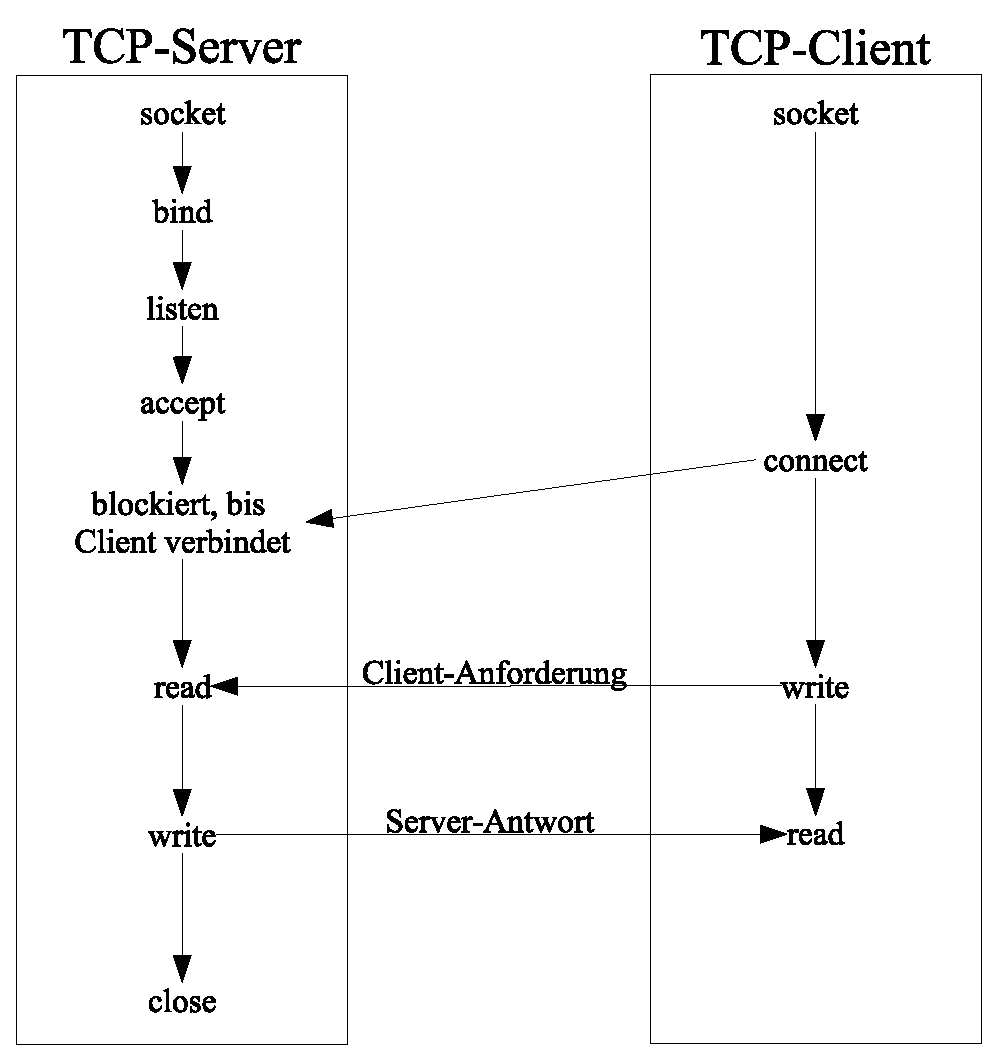
\includegraphics[width=10cm]{images/tcpsocket.eps}
        \caption{Ablauf TCP-Socket}
        \label{fig:tcpsocket}
      \end{figure}
      Als erstes muss der Socket erstellt werden. Mit \emph{bind} wird dieser Socket 
      an eine bestimmte Portnummer gebunden und mit dem Befehl \emph{listen} wird 
      dem Socket mitgeteilt, das er auf Verbindungsversuche zu dieser Portnummer 
      lauschen soll. Jetzt wartet der Server mit \emph{acceppt} auf einen 
      Verbindungsversuch des Clients. Dies ist entweder als blockierende oder
      nicht blockierende Funktion implementiert (siehe Abschnitt \ref{blocksocktets}). 
      Nach dem \emph{accept} die Verbindung akzeptiert hat, wird der normale
      Kommunikationsprozess durchgef�hrt. Als erstes liest der Server (\emph{read}) die Anfrage
      vom Client und schickt eine Antwort (\emph{write}) an den Client zur�ck.
      Danach ist vom Server die Verbindung zu beenden (\emph{close}).


    \subsection{Blockierende und nicht blockierende Sockets}
      \label{blocksocktets}  
  
      Gewisse Funktionen einer Socketoperation k�nnen als blockierende oder nicht blockierende 
      Operation ausgef�hrt werden. Blockierend bedeutet, dass die Funktion so lange wartet,
      d.h. dass das restliche Programm an dieser Stelle unterbrochen wird, 
      bis die Aktion ausgef�hrt wurde. Eine typische Operation ist das Warten auf eine
      Anfrage vom Client. In dieser Zeit ist der Prozess stillgelegt, bis eine Anfrage 
      auf dem Kommunikationskanal anliegt. So lange der Prozess wartet, wird keine
      Prozessorleistung verbraucht. Andere Prozesse auf 
      dem Rechner k�nnen normal weiterarbeiten, da der Prozessor keine Belastung durch das
      Warten auf eine Anfrage hat. Wenn diese Operation als nicht blockierende 
      Operation realisiert w�re, so w�rde, wenn kein Anfragesignal auf dem 
      Kommunikationskanal anliegt, die Funktion an dieser Stelle nicht warten, sondern einfach 
      im Programm weitermachen. Um nun eine Anfrage �ber das Socket zu registrieren, ist die Ausf�hrung 
      der Operation in einer Endlosschleife n�tig. Dies verbraucht aber viele Ressourcen des Prozessors.
      Auf Grund der Performance des Gesamtsystems sind also blockierende Sockets vorzuziehen.
